\section{Conclusion}

Computation of midsurface is one of the popular simplification techniques for CAE analysis of  thin-walled models. In-spite of good demand, current methods (especially the popular Midsurface Abstraction - MA) suffer from problems such as gaps, overlaps, not lying midway, improper connections, etc.  In MA, these failures are due to complexities of face-pair detection and interactions. In our approach uses feature simplification and abstraction to resolve face-pair detection problems and  cellular decomposition to develop a generic logic to address interaction problems amongst midsurface patches. 

%\vspace{-5mm}

\begin{figure}[htp]
\centering     %%% not \center
\subfloat[Original Part]{\label{fig_orig}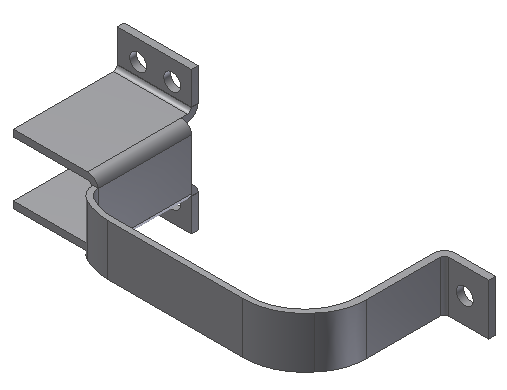
\includegraphics[width=0.23\linewidth,valign=t]{../images/nonCellularBracket}} \quad
\subfloat[Decomposition]{\label{fig_cd}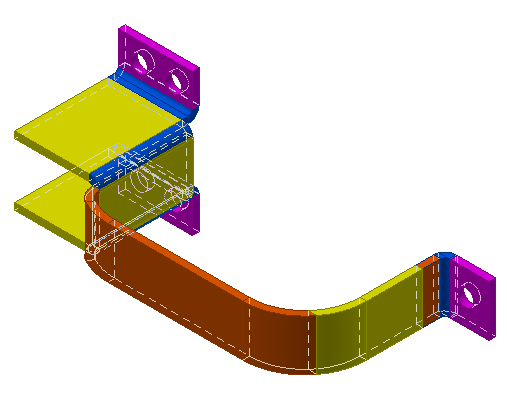
\includegraphics[width=0.23\linewidth,valign=t]{../images/CellularBracket}}\quad
\subfloat[Graph]{\label{fig_cg}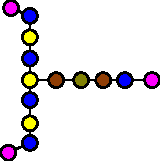
\includegraphics[width=0.175\linewidth,valign=t]{../images/CellGraphBracket.pdf}} \quad
\subfloat[Midsurface]{\label{fig_mids}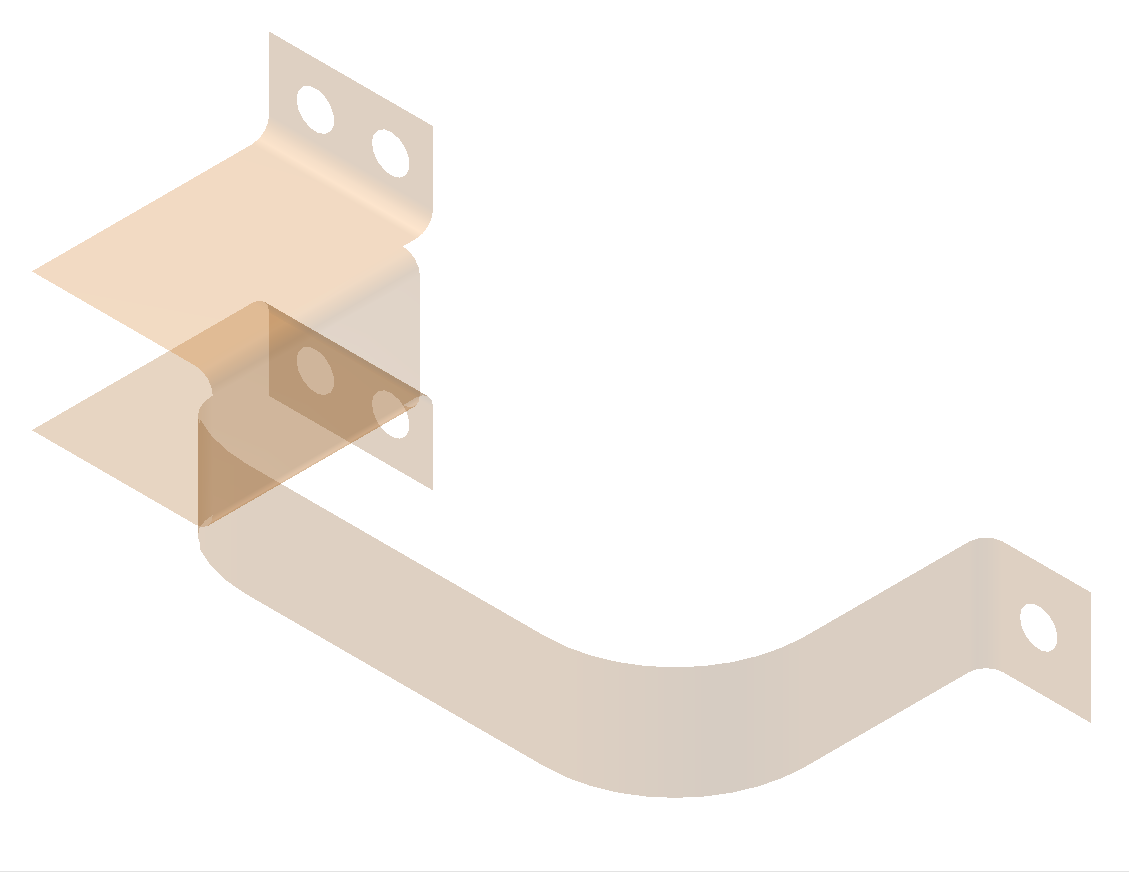
\includegraphics[width=0.23\linewidth,valign=t]{../images/MidsurfAfterDormant}}
\end{figure}


Following is a  comparative analysis of some relevant approaches vis-a-vis our approach:

\begin{table}[htp]
%\tiny
  \centering 
\resizebox{0.8\linewidth}{!}{ 
\begin{tabular}[htp]{@{} p{0.1\linewidth} p{0.2\linewidth}  p{0.2\linewidth} p{0.2\linewidth} p{0.2\linewidth}@{}}
\toprule
\textbf{Researcher}  &	\textbf{Method} &	 \textbf{Shortcomings}  &	 \textbf{Our Approach}\\ \midrule
\textbf{Chong et al.} \cite{Chong2004}  & 
Uses concave edge decomposition. Midcurves by collapsing edge pairs. If they form a loop, creates a midsurface patch & 
Hard-coded inequalities/values to detect edge-pairs. Connection logic is not generic and comprehensive &
A generic treatment for the computation of midcurves, midsurface patches and their connections
\\ \midrule
 \textbf{Boussuge et al.} \cite{Boussuge2014}  & 
 Generative decomposition. Recognizes Extrudes of each sub-volume. Creates midsurface patches in each and connects them together. &
 
 \begin{itemize}[noitemsep,nosep,leftmargin=*]
\item No fillets/chamfers.
\item Only Additive cells.
\item Only Extrudes with Analytical surfaces
\item Expensive MAT to detect thin profiles
\item Works only on Parallel and Orthogonal connections.
\end{itemize}
&
\begin{itemize}[noitemsep,nosep,leftmargin=*]
\item No such restriction
\item Re-inserts -ve cells
\item Generic Sweep extend-able to Loft
\item Simple rules of size of profile/guide
\item Generic logic for any numbers/types of connections.
\end{itemize}

\\ \midrule

\end{tabular}
}
% \caption{Comparison with Other Simplification Methods}
%  \label{tab:defeat_test}
\end{table}


%\vspace{-8mm}
